% This is samplepaper.tex, a sample chapter demonstrating the
% LLNCS macro package for Springer Computer Science proceedings;
% Version 2.21 of 2022/01/12
%
\documentclass[runningheads]{llncs}
%
\usepackage[T1]{fontenc}
% T1 fonts will be used to generate the final print and online PDFs,
% so please use T1 fonts in your manuscript whenever possible.
% Other font encondings may result in incorrect characters.
%
\usepackage{amsmath}
\usepackage{graphicx}
\usepackage{amssymb}
\usepackage{algorithm}
\usepackage{algpseudocode}
\usepackage{tikz}
\usepackage{fixme}
\usepackage{url}
\usepackage{booktabs}
\usetikzlibrary{arrows.meta, positioning}
\fxsetup{status=draft} % <====== add this line
 
\usepackage{graphicx}
\usepackage{subcaption}

% Used for displaying a sample figure. If possible, figure files should
% be included in EPS format.
%
% If you use the hyperref package, please uncomment the following two lines
% to display URLs in blue roman font according to Springer's eBook style:
%\usepackage{color}
%\renewcommand\UrlFont{\color{blue}\rmfamily}
%\urlstyle{rm}
%
\begin{document}
	
	\title{On Solving the Multiple Variable Gapped Longest Common Subsequence Problem}
	%
	\titlerunning{On Solving the MVGLCSP}
	
	\author{
		Marko Djukanović\inst{1,2, 6}  \and
		Nikola Balaban\inst{2}   \and
		Christian Blum\inst{3}  \and 
		Aleksandar Kartelj\inst{4}  \and
		Sašo Džeroski\inst{5}  \and
		Žiga Zebec\inst{6}
	}
	%
	\authorrunning{Djukanovic et al.}
	
	\institute{		University of Nova Gorica, Nova Gorica, Slovenia \\ \email{marko.dukanovic@ung.si} \\ \and Faculty of Natural Sciences and Mathematics, University of Banja Luka, Banja Luka, Bosnia and Herzegovina \\
		\email{nikola.balaban@student.pmf.unibl.org}, \email{marko.djukanovic@pmf.unibl.org} \and
		Artificial Intelligence Research Institute (IIIA-CSIC), Barcelona, Spain \\
		\email{christian.blum@iia.csic.es} \and 
		Faculty of Mathematics, University of Belgrade, Belgrade, Serbia \\ \email{kartelj@matf.rs} \\ \and
		Jožef Stefan Institute, Ljubljana, Slovenia \ \\ \email{saso.dzeroski@ijs.si}  \\
		\and
		Institute of Information Sciences (IZUM), Maribor, Slovenia \\
		\email{ziga.zebec@izum.si}
	}
	%
	\maketitle              % typeset the header of the contribution
	%
	\begin{abstract}
This paper addresses the Variable Gapped Longest Common Subsequence (VGLCS) problem, a generalization of the classical longest common subsequence (LCS) problem to an arbitrarily large set of input strings under flexible gap constraints. The problem arises in applications such as molecular sequence comparison, where structural distance constraints between nucleotides must be respected, and time-series analysis, in which events are required to occur within specified temporal delays. We propose a novel solution framework based on a root-based state graph representation, in which the overall state space is defined as the union of a potentially large number of root-based state graphs. To cope with the resulting combinatorial explosion, we introduce an iterative beam search strategy that dynamically maintains a global pool of promising candidates for root nodes, enabling effective control of diversification across iterations. To further guide the search, several heuristic evaluation functions inspired by the LCS literature are incorporated into the standalone beam search procedure. To the best of our knowledge, this work presents the first comprehensive computational study of the VGLCS problem, using a benchmark of 320 synthetic instances. Experimental results show that the proposed iterative beam search consistently outperforms both a baseline beam search and an iterative greedy approach within comparable computational times. Furthermore, in the special case of two input strings, the proposed method achieves performance comparable to three specialized dynamic programming algorithms on small-to-medium-sized instances, while significantly outperforming two alternative heuristic variants.
	\keywords{Longest common subsequences  \and Beam Search  \and Bioinformatics \and Gap constraints}
	\end{abstract}
	%
	%
	%
    \section{Introduction}
	
The \textit{Longest Common Subsequence Problem} (LCSP)~\cite{DJUKANOVIC2020106499,bergroth2000survey} is a well-known combinatorial optimization problem with numerous applications in bioinformatics and computational biology, where it plays a fundamental role in the analysis and comparison of molecular sequences. Given an arbitrarily large set of input sequences
\[
S=\{s_1,\ldots,s_m\}, \quad m \in \mathbb{N},
\]
defined over an alphabet $\Sigma$, the objective is to identify a longest possible subsequence that is common to all sequences $s_i \in S$.

Over the past decades, a variety of practically motivated extensions of the LCSP have been proposed to better capture structural, biological, or application-specific requirements. Notable variants include constrained, arc-preserving, and repetition-free longest common subsequence problems~\cite{jiang2004longest,farhana2015constrained,adi2010repetition}, among others.

In this work, we focus on the \textit{Variable Gapped Longest Common Subsequence Problem} (VGLCSP), which was originally introduced for the case of two input strings in~\cite{penga2011longest} and further investigated from a theoretical perspective in~\cite{adamson2023longest}. The VGLCSP extends the classical LCSP by incorporating flexible distance constraints (referred to as \emph{gaps}) between consecutive symbols of the resulting subsequence. Unlike fixed-gap models, these gap limits are allowed to vary along the input sequences, thereby offering increased modeling flexibility.

Formally, for each input sequence $s_i \in S$, a gap constraint is defined by a function
\[
G_i \colon \{1,\ldots,|s_i|\} \mapsto \mathbb{N}.
\]
If the characters of a common subsequence $s$ occur at positions
$i^1_i < \cdots < i^{|s|}_i$ in sequence $s_i$, then the gap constraint is satisfied if
\[
i^x_i - i^{x-1}_i \leq G_i[i^x_i] + 1, \quad x = 2,\ldots,|s|.
\]
A common subsequence is considered \emph{feasible} if the corresponding gap constraints are satisfied simultaneously for all sequences in $S$.

The VGLCSP provides a flexible and realistic model for sequence comparison, particularly suited to applications in DNA and protein analysis where variable structural distances between residues must be respected. Beyond bioinformatics, the problem also arises in time-series analysis, especially in settings where events are required to occur within specified temporal delays~\cite{lainscsek2015delay}.
 \fxnote{Give an example of an VGLCS problem instance with solution ... }
	
	Although several exact dynamic programming approaches exist for the two-sequence case ($m=2$)~\cite{penga2011longest}, their computational complexity becomes prohibitive for larger $m$. To the best of our knowledge, no effective exact or approximate approaches are currently existing for the generalized VGLCSP with arbitrary large set $S$, which is clearly an NP-hard problem as a general version of the LCS problem with arbitrary large set of input strings. 
	
	\subsection{Preliminaries and Notation}
	  
	Before introducing the algorithmic framework for the problem under consideration, we first define the notation used throughout this work.
	
	Let $|s|$ denote the length of a sequence $s$. The symbol $s[i]$ refers to the character at position $i$ of sequence $s$, where indexing starts at $i = 1$. The substring of $s$ that begins at position $i$ and ends at position $j$ is denoted by $s[i,j]$. If $i = j$, this substring corresponds to the single character $s[i]$; if $j < i$, then $s[i,j] = \varepsilon$, where $\varepsilon$ denotes the empty string.
	
	The number of occurrences of a character $a \in \Sigma$ in a sequence $s$ is denoted by $|s|_a$. For a subset of characters $\Sigma' \subseteq \Sigma$, the number of occurrences of characters from $\Sigma'$ in $s$ is defined as
	\[
	|s|_{\Sigma'} = \sum_{\sigma \in \Sigma'} |s|_{\sigma}.
	\]
	
	We denote by $S = \{s_1, \ldots, s_m\}$ the set of input sequences. Unless stated otherwise, $m \in \mathbb{N}$ represents the number of input sequences (and, correspondingly, the number of gap constraints), and $n$ denotes the length of the longest sequence in $S$.
	
	The remainder of the paper is organized as follows. Section~\ref{sec: state_graph} introduces the state graph representation of the problem. In Section~\ref{sec: imsbs}, we present the design of our main methodological contribution, namely the iterative multi-source beam search approach. Section~\ref{sec: experiments} reports the computational results, comparing the proposed method with a baseline standalone beam search and a greedy heuristic, as well as with specialized approaches for the case of two input sequences. Finally, Section~\ref{sec: conclusions} concludes the paper and outlines directions for future research.
	
	
	\section{Root-based State Space Formulation}\label{sec: state_graph}
	
     Building on the state-space representation for the LCSP introduced in~\cite{DJUKANOVIC2020106499}, we develop a \emph{root-based state graph} model for the Variable Gapped Longest Common Subsequence Problem (VGLCSP). Each state represents one or more feasible partial solutions characterized by a vector of positions induced by the input sequences and by the current subsequence length.
     
     Formally, a partial subsequence $s^v$ induces a state node
     \[
     v = (\mathbf{p}^{L,v},\, l^v),
     \]
     where $\mathbf{p}^{L,v} = (p^{L,v}_1,\ldots,p^{L,v}_m)$ and the following conditions hold:
     (i) for each sequence $s_i \in S$, the index $p^{L,v}_i - 1$ is the smallest position such that $s^v$ is a subsequence of $s_i[1,\, p^{L,v}_i - 1]$;
     (ii) $l^v = |s^v|$ denotes the length of the partial subsequence; and
     (iii) all gap constraints $G_i$ are satisfied by $s^v$ with respect to every input sequence $s_i$.
     
     A directed arc $\alpha = (v_1, v_2)$, labeled with $lett(\alpha) = a \in \Sigma$, exists if
     \[
     l^{v_2} = l^{v_1} + 1
     \quad \text{and} \quad
     s^{v_2} = s^{v_1} \cdot a,
     \]
     that is, state $v_2$ corresponds to extending a partial solution of $v_1$ by appending the character $a$.
     
     To expand a state $v$, only those characters $a \in \Sigma$ that occur in the suffix of each sequence $s_i$ starting at position $p^{L,v}_i$, for $i = 1,\ldots,m$, are considered. For each such character $a$, we identify the smallest feasible positions $p^{L,a}_i \ge p^{L,v}_i$ such that
     \[
     s_i[p^{L,a}_i] = a
     \quad \text{and} \quad
     p^{L,a}_i - p^{L,v}_i \le G_i(p^{L,a}_i),
     \qquad i = 1,\ldots,m.
     \]
     If such positions exist for all sequences, a child state
     \[
     w = (\mathbf{p}^{L,a} + \mathbf{1},\, l^v + 1)
     \]
     is generated, unless it is dominated by another child state according to the dominance criteria defined later.
     
     To efficiently compute child states and their associated position vectors, we employ a preprocessing data structure denoted by \texttt{Succ}. This structure is a three-dimensional integer array indexed by $(i,j,a)$, where $i$ refers to the input sequence $s_i$, $1 \le j \le |s_i|$ denotes a position within that sequence, and $a \in \Sigma$ is a character. The value
     \[
     q = \texttt{Succ}[i,j,a]
     \]
     stores the smallest index $q \ge j$ such that $s_i[q] = a$ and the gap constraint is satisfied at position $q$, that is,
     \[
     q - j \le G_i(q).
     \]
     If no such position exists, the value $-1$ is assigned.
     
     The root state is defined as
     \[
     r = ((1,\ldots,1),\, 0),
     \]
     corresponding to the empty subsequence. Goal states are feasible states that cannot be further expanded. The search space rooted at $r$ is denoted by $\mathrm{Space}(r)$. As discussed in the following section, the structure of this space depends on the choice of the root state from which the search is initiated.
     
     
% U nekom delu LaTeX dokumenta:
\begin{figure}[h!]
	\centering
	\scalebox{0.4}{
	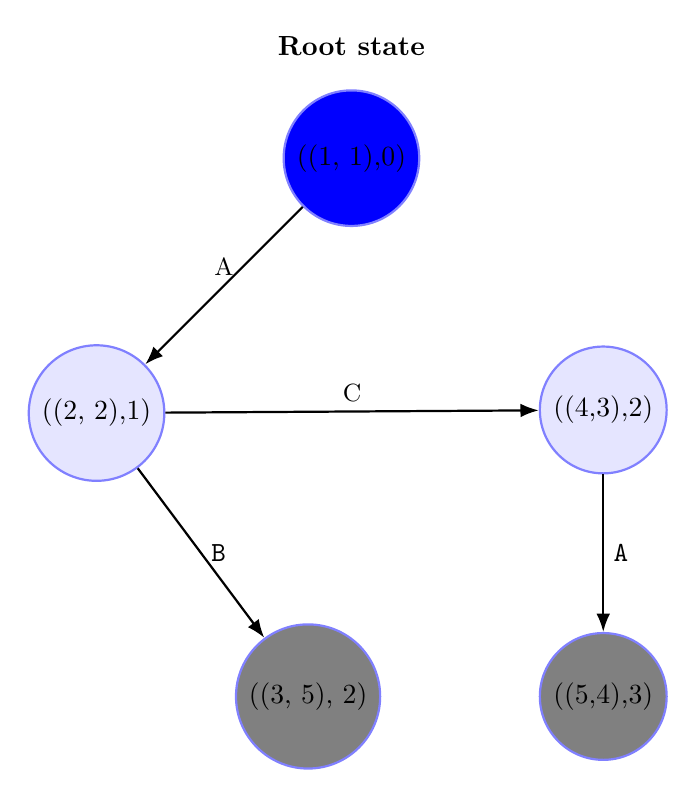
\begin{tikzpicture}[
		state/.style={circle, draw=blue!50, fill=blue!10, thick, minimum size=8mm},
		edge/.style={-Latex, thick},
		node distance=2cm and 2cm
		]
		
		% Čvorovi
		\node[state, fill=blue] (s0) {((1, 1),0)};
		\node[state, below left=of s0] (s1) {((2, 2),1)};
		\node[state, below right=of s0] (s2) {((4,3),2)};
		%\node[state, below=of s2] (s3) {(4,3)};
		\node[state, below=of s2, fill=gray] (s4) {((5,4),3)}; % krajnje, ali ne koristi se ovde
		\node[state, left=of s4, fill=gray] (s5) {((3, 5), 2)}; % krajnje, ali ne koristi se ovde
		
		% Grane (samo validne poklapanja)
		\draw[edge] (s0) -- node[above] {\small A} (s1);
		%\draw[edge] (s0) -- node[above] {\small A} (s2);
		\draw[edge] (s1) -- node[above] {\small C} (s2);
		%\draw[edge] (s2) -- node[right] {\small A} (s3);
		%\draw[edge] (s3) -- node[right] {\texttt{A}} (s4);
		\draw[edge] (s1) -- node[right] {\texttt{B}} (s5);
		% Oznake
		\node[above=0.3cm of s0] {\textbf{Root state}};
		%\node[below=1.5cm of s3] {\small \textbf{Krajnje stanje}};
		\draw[edge] (s2) -- node[right] {\texttt{A}} (s4);
		
	\end{tikzpicture}}
	\caption{State graph $Space(((1, 1), 0))$ for MVGLCSP between the sequences \texttt{ABCA} i \texttt{ACAB}. Two final/terminal states are displayed in gray. }
	\label{fig:vgcs-grafstanja}
\end{figure}

\paragraph{Motivation for Multi-Source Beam Search.}
Unlike the classical LCSP, the VGLCSP may exhibit multiple, potentially exponentially many, \emph{disconnected root components} in its state space. Consequently, a search strategy that expands states from a single initial root may fail to reach feasible and even optimal solutions.

As an illustrative example, consider the sequence set
\[
S = \{ s_1 = \texttt{ATGGAAAA},\; s_2 = \texttt{ATCCAAAA} \},
\]
with gap constraints $G_{s_1} = G_{s_2} = 1$, depicted in Fig.~\ref{fig:vgcs-grafstanja}. In this instance, the initial state $((1,1),0)$ cannot reach any state with position vector $\mathbf{p}^L = (5,5)$ via standard directed transitions. As a result, the optimal common subsequence \texttt{AAA} is unreachable when the search is initiated exclusively from the initial root state $((1,1),0)$, and is therefore missed by traditional search strategies.

To address this issue, the full state space of a VGLCSP instance is naturally defined as
\[
\bigcup_{q \in \mathcal{R}} \mathrm{Space}(q),
\]
where $\mathcal{R}$ denotes the set of all root states, i.e., states with position vectors $\mathbf{p}^{L,q}$ that cannot be reached from any other state through regular directed transitions. However, explicitly enumerating all such root states is computationally prohibitive in general, requiring $O(n^m)$ time in the worst case, and is thus infeasible for instances with large $m$ or $n$.

This structural characteristic of the VGLCSP motivates the proposed \textit{Iterative Multi-Source Beam Search} (IMSBS) approach, which is specifically designed to dynamically explore multiple promising regions of the state space. By iteratively identifying and expanding a set of candidate root states, IMSBS effectively mitigates the disconnection effects induced by gap constraints and enables the discovery of high-quality solutions that would otherwise remain inaccessible to single-source search methods.


	
	\section{Iterative Multi-source Beam Search Framework}\label{sec: imsbs}
	
\textit{Beam search} (BS) is a well-established tree-search metaheuristic that operates in a breadth-first-search manner. The search is controlled by a beam width parameter $\beta$, which specifies the maximum number of nodes retained for expansion at each level, and by a heuristic evaluation function $h$, which guides the selection of the most promising nodes for further expansion.

Within the \textit{Iterative Multi-Source Beam Search} (IMSBS) framework, BS is executed iteratively, each time initialized with a beam $\mathcal{L}$ consisting of several promising root nodes. These root nodes are dynamically selected from a global pool $\mathcal{R}$, whose role is to promote diversification across different regions of the state space. Each BS execution thus explores the neighborhood of multiple starting points rather than relying on a single root.

The beam search itself employs several heuristic components to intensify the search toward high-quality feasible solutions. These heuristics include estimates based on letter frequencies, minimal residual substring lengths, and probability-weighted bounds, which are described in detail in the subsequent sections.

The overall procedure is summarized in Algorithm~\ref{alg:imbs}. Initially, the pool of root nodes $\mathcal{R}$ is initialized with the root state $r = ((1,\ldots,1), 0)$, corresponding to the empty partial solution, and the current best solution is set to $s_{\mathrm{best}} = \varepsilon$. The algorithm iterates until either the pool $\mathcal{R}$ becomes empty or a predefined maximum number of beam search calls is reached.

At each iteration, a fixed number of the most promising root nodes from $\mathcal{R}$—controlled by the parameter \emph{number\_of\_sources\_from\_R} and ranked according to a heuristic evaluation $h'$—are extracted and stored in a temporary beam $\mathcal{L}$. This beam serves as the initial point for the current beam search, which is executed using beam width $\beta$ and heuristic guidance function $h$.

During the beam search, all completed (i.e., non-expandable) nodes are processed as follows. If a completed node corresponds to a solution that improves upon the current best, the incumbent solution $s_{\mathrm{best}}$ is updated accordingly. Each completed node is then independently expanded in an LCS-like manner, ignoring gap constraints, to generate a set of successor nodes. For a generated child node $w$ with position vector $\mathbf{p}^w$, if
\[
|s_i| - p^w_i + 1 \leq |s_{\mathrm{best}}|
\quad \text{holds for at least one } i \in [m],
\]
the node is discarded as it cannot lead to an improvement over the current best solution. Otherwise, a corresponding root candidate $r^w = (\mathbf{p}^w, 0)$ is inserted into the pool $\mathcal{R}$, provided that it has not already been part in the previous iterations.

Once the current beam search terminates, a new iteration is initiated with a freshly selected set of root nodes from $\mathcal{R}$, as long as the termination conditions are not met. The pool $\mathcal{R}$ is maintained as a priority queue implemented via a binary heap, ensuring efficient extraction of the most promising root nodes.

     
    
    %pseudocode:
    \begin{algorithm}[!ht]
    	\caption{Iterated Multi-source Beam Search (IMSBS) Framework }
    	\label{alg:imbs}
    	\begin{algorithmic}[1]
    		\Require Sequences $s_1, \dots, s_m$; Gap functions $G_{s_i}(\cdot)$; beam width $\beta>0$; ${number\_sources\_from\_R}>0$; $beam\_iters>0$, heuristics $h, h'$
    		\Ensure Approximate common subsequence $s_{\textrm{best}}$
    		
    		\State Initialize $\mathcal{R} \gets \{ (\mathbf{1},0) \}$ \Comment{A set of root nodes}
    		\State $iter \gets 0$
    		\State $s_{\textrm{best}} \gets  \varepsilon$
    		
    		\While{$\mathcal{R} \neq \emptyset \wedge iter < beam\_iters $ }
    		\State Select $\mathcal{L} \subseteq \mathcal{R}$  ${number\_sources\_from\_R}$ nodes, \State Remove the selected nodes from $\mathcal{R}$
    		\Comment{$\mathcal{R}$ can be a pr. queue ordered by heuristic $h'$}
    		\State Execute beam search $BS( \mathcal{L}, h)$
    		
    		\ForAll{complete nodes $v$ at $BS(\mathcal{L}, h)$}
    		\ForAll{Symbol $a \in \Sigma$}
    		\State $p^w \gets$ minimum positions in the sequences so that $\ge p^v$ and $s_i[p^w_i] = a$ (ignore all gap constraints)
    		\If{$|s_{\textrm{best}}| < \min_{i=1,\dots,m} \{ |s_i| - p^w_i + 1 \}$}    \Comment{cut-off}
    		\State Add $r^w = (p^w,0)$ in the set  $\mathcal{R}$ (if previously have not added)
    		\EndIf
    		\EndFor
    		\EndFor
    		
    		\State Update $s_{\textrm{best}}$ if a new longest subsequence  in $BS(\mathcal{L}, h)$ has been found
    		\State $iter \gets iter + 1$
    		\EndWhile
    		
    		\State \Return $s_{\textrm{best}}$
    	\end{algorithmic}
    \end{algorithm}
    The core advantages of the IMSBS approach over the baseline BS are: 
    \begin{itemize}
    	\item It provides a heuristic balance between beam search (local exploration of promising paths) and the generation of new sources (global coverage of the search space).
    	\item Filtering suboptimal root nodes reduces unnecessary iterations and enables pruning of dominated paths.
    \end{itemize}

    \subsection{Heuristic guidances}
    
    Several heuristics to guide search are utilized within the IMSBS (as the candidate for $h$ and $h'$). 
    \begin{itemize}
    	\item  \textit{``Look-ahead'' for the remaining length:}
    	\begin{equation}
    		\textrm{UB}_1(\mathbf{v}) = \min_{i = 1, \ldots, m} \left( |s_i| - p_i^v + 1 \right)
    	\end{equation}
    	This is an estimate of the potential extension of the sequence up to the end of the shortest remaining sequence.
    	
    	\item  \textit{Character Frequency Alignment:}
    \begin{equation}
    	\textrm{UB}_2(\mathbf{v}) =  \sum_{\sigma \in \Sigma} 
    	\min\left(  |s_1[p_1^v, |s_1|]|_{\sigma}, \ldots, |s_m[p_m^v, |s_m|]|_{\sigma} \right)
    \end{equation}
    In essence, this heuristic counts the maximum number of characters that can still match in the (optimal) solution based on the frequency of each character. This score can be computed efficiently in \(O(m)\) time using preprocessing (i.e., constructing suitable data structures), see~\cite{DJUKANOVIC2020106499}. 
     \item \textit{A probability-based heuristic} guidance by the Mousavi and Tabataba's matrices from~\cite{mousavi2012improved} in the context of the LCS problem. These probabilities are based on the idea of determining a probability for the event realization that a sequence $s$ of length $k$ is a subsequence of a (random) sequence of length $n$ over an alphabet $\Sigma$.  The probabilities for each  $i=1,\ldots, k$ and  $j=1, \ldots, n$, are pre-processed by a matrix $\mathcal{P}$ of probabilities of dimension $k\times n$ by a dynamic programming recurrence. Assuming the independence betwen input sequences, at each level of beam search the nodes are evaluated by determining the probabilities for each partial solutions  across that level to be expanded by $\overline{k}$ letters (this value is heuristically evaluated, as proposed in~\cite{mousavi2012improved}). Denote that heuristic guidance   by $h_{\textrm{prob}}$. 
     \item TODO: \fxnote{TODO: if we come up with some learning heuristic -- should left for the extended version -- journal-extendable.}
   \end{itemize}
    
	
\section{Experimental Evaluation}\label{sec: experiments}
   
In this section, we compare the performance of heuristic approaches designed for the VGLCSP with an arbitrary number of sequences \( m \geq 2 \). Specifically, we consider the following methods:

\begin{itemize}
	\item \textsc{Bs}: a baseline beam search approach that starts from the root node \( r \) as the initial beam and performs a single iteration of IMSBS.
	
	\item \textsc{Imsbs}: a tuned iterative multi-source beam search, described in Algorithm~\ref{alg:imbs}, configured to use a runtime comparable to that of \textsc{Bs}.
	
	\item \textsc{Imsbs-greedy}: a variant of IMSBS with a fixed parameter \( \beta = 1 \), as given in Algorithm~\ref{alg:imbs}. This configuration highlights the impact of performing a larger number of beam search iterations on the overall performance of \textsc{Imsbs}.
\end{itemize}

The \textsc{Imsbs} algorithm is implemented in Python~3.11 and evaluated on the VEGA high-performance computing system hosted at IZUM, Maribor. The cluster consists of 960 compute nodes equipped with AMD EPYC 7H12 CPUs operating at 2.35\,GHz. All experiments were conducted in a single-threaded setting.

   
 \subsection{Instance generation}
 
 For each combination of instance parameters $n \in \{50, 100, 200, 500\}$, $m \in \{2, 3, 5, 10\}$, and $|\Sigma| \in \{2, 4\}$, we generate 10 random problem instances. First, $m$ sequences of equal length are generated uniformly at random. Then, the gap constraints for each instance (i.e., positions within sequences) are generated such that for each $G_i(j), j=1, \ldots, |s_i|, i=1, \ldots, m$, a value 
 $G_{s_i}(j) \in \mathcal{U}(\{ \lfloor 0.5 \cdot |\Sigma| \rfloor, \ldots, \lfloor 1.5 \cdot |\Sigma| \rfloor \})$ is assigned.  Therefore, a total of 320 problem instances are generated. The benchmark set is denoted as \textsc{Random}. All instances from the \textsc{Random} dataset can be found at   
 \url{https://github.com/markodjukanovic90/NikolaBalabanDiplomski/tree/main/src/instance_i_generator}.
 
 \subsection{Parameter tuning}
 
 For the \textsc{Bs} approach, a high beam width $\beta = 10,000$ and $h = h_{\text{prob}}$ are used, as further increasing the beam size does not significantly improve solution quality. The heuristic $h_{\text{prob}}$ provides slightly better guidance than $\textrm{UB}_2$ and significantly better than $\textrm{UB}_1$; see Fig.~\ref{fig:bs_tuning}.
 
 \begin{figure}[!ht]
 	\centering
 	\begin{subfigure}[t]{0.48\textwidth}
 		\centering
 		\includegraphics[width=\linewidth, height=120pt]{figures/bs_tuning_quality.png}
 		\caption{Avg. quality over all instances from the \textsc{Random} benchmark suite.}
 		\label{fig:tune_bs}
 	\end{subfigure}
 	~
 	\begin{subfigure}[t]{0.48\textwidth}
 		\centering
 		\includegraphics[width=\linewidth, height=120pt]{figures/bs_tuning_time.png}
 		\caption{Avg. runtime over all instances from the \textsc{Random} benchmark suite.}
 		\label{fig:tune_bs_time}
 	\end{subfigure}
 	\caption{Beam search tuning results on the \textsc{Random} benchmark suite.}
 	\label{fig:bs_tuning}
 \end{figure}
 
 After preliminary experiments, we fixed ${\text{number\_sources\_from\_R}} = 10$ and \emph{beam\_iters} = 50, as high-quality results were already achieved with this number of iterations. Root nodes kept in the global set are prioritized according to $h' = \textrm{UB}_2$, which consistently improves IMSBS performance compared to using $\textrm{UB}_1$.    The remaining parameters of the IMSBS approach were tuned via a simple grid search over the following values: $h \in \{\textrm{UB}_1, \textrm{UB}_2, h_{\text{prob}}\}$ and $\beta \in \{100, 500, 2000\}$, see Fig.~\ref{fig:imsbs_tuning}.
 
 \begin{figure}[!h]
 	\centering
 	\begin{minipage}{0.48\textwidth}
 		\centering
 		\includegraphics[width=\linewidth]{figures/imsbs_tuning.png}
 		\caption*{(a) Avg. quality for different IMSBS settings over all instances from the \textsc{Random} benchmark suite.}
 		\label{fig:tune_imsbs}
 	\end{minipage}
 	~
 	\begin{minipage}{0.48\textwidth}
 		\centering
 		\includegraphics[width=\linewidth]{figures/imsbs_tuning_time.png}
 		\caption*{(b) Avg. runtime for different IMSBS settings over all instances from the \textsc{Random} benchmark suite.}
 		\label{fig:tune_imsbs_time}
 	\end{minipage}
 	\caption{IMSBS parameter tuning results on the \textsc{Random} benchmark suite.}
 	\label{fig:imsbs_tuning}
 \end{figure}
 
 To ensure comparable average runtime between IMSBS and the baseline \textsc{Bs} approach, we use the following IMSBS configuration in our experiments: $h = \textrm{UB}_2$ and $\beta = 500$. These values balance runtime relative to \textsc{Bs} while maintaining reasonable solution quality.  
 
 Similarly, for the \textsc{Imsbs-greedy} approach with fixed $\beta = 1$, we allow a budget of 5000 beam search iterations (\emph{beam\_iters} = 5000), while all other parameters remain the same as for \textsc{Imsbs}.
 
  
  \subsection{Numerical results for heuristic approaches }
  Numerical results for all three heuristic approaches are reported in Table~\ref{tab:numerical_results_general_m}, which is organized into two main parts. 
  The first three columns describe the instance characteristics: the number of sequences ($m$), the sequence length ($n$), and the alphabet size ($|\Sigma|$). 
  The remaining columns report the performance of the three heuristic approaches: \textsc{Bs}, \textsc{Imsbs-greedy}, and \textsc{Imsbs}.  
  
  For each algorithm, two performance indicators are provided: the average objective value $\overline{obj}$ and the average running time in seconds $\overline{t}$, computed over 10 instances per group. 
  This layout allows a direct comparison of solution quality and computational effort across algorithms under identical instance settings.
  
    
    
    \begin{table}[H]
    	\caption{Numerical results of the three heuristic approaches on the \textsc{Random} benchmark suite. }\label{tab:numerical_results_general_m}
    	\centering
    	\scalebox{0.8}{
    	\begin{tabular}{lll|rr|rr|rr}
    		\hline
    		\multicolumn{3}{c}{Inst.} & \multicolumn{2}{c}{\textsc{Bs}} & \multicolumn{2}{c}{\textsc{Imsbs-Greedy}} & \multicolumn{2}{c}{\textsc{Imsbs}} \\
    		\cmidrule(lrr){1-3} \cmidrule(lr){4-5} \cmidrule(lr){6-7} \cmidrule(lr){8-9} \\ 
    		$m$ & $n$ & $|\Sigma|$ & $\overline{obj}$ & $\overline{t}[s]$ & $\overline{obj}$ & $\overline{t}[s]$ & $\overline{obj}$ & $\overline{t}[s]$ \\
    		\hline
\midrule
   2 & 50 & 2 & 33.6 & 0.02 & 26.1 & 0.00 & \textbf{35.0} & 0.04 \\
   2 & 50 & 4 & 30.1 & 0.89 & 24.8 & 0.00 & \textbf{30.1} & 0.14 \\
   2 & 100 & 2 & 48.9 & 1.74 & 41.5 & 0.00 & \textbf{65.1} & 0.44 \\
   2 & 100 & 4 & \textbf{62.1} & 9.75 & 50.5 & 0.00 & 61.6 & 0.67 \\
   2 & 200 & 2 & 99.1 & 14.76 & 67.7 & 0.01 & \textbf{123.3} & 3.20 \\
   2 & 200 & 4 & 120.5 & 38.56 & 74.8 & 0.01 & \textbf{120.9} & 3.55 \\
   2 & 500 & 2 & 65.3 & 21.05 & 77.3 & 0.03 & \textbf{184.9} & 62.69 \\
   2 & 500 & 4 & 214.6 & 155.30 & 152.4 & 0.02 & \textbf{222.8} & 35.27 \\ \hline
   
   3 & 50 & 2 & 17.5 & 0.02 & 17.4 & 0.00 & \textbf{25.8} & 0.05 \\
   3 & 50 & 4 & \textbf{21.7} & 0.17 & 16.1 & 0.00 & \textbf{21.7} & 0.09 \\
   3 & 100 & 2 & 19.7 & 0.07 & 25.2 & 0.00 & \textbf{46.6} & 1.42 \\
   3 & 100 & 4 & 34.1 & 2.50 & 21.1 & 0.00 & \textbf{42.3} & 2.49 \\
   3 & 200 & 2 & 15.2 & 0.15 & 29.2 & 0.01 & \textbf{73.6} & 9.63 \\
   3 & 200 & 4 & 85.3 & 24.99 & 38.3 & 0.01 & \textbf{91.3} & 33.44 \\
   3 & 500 & 2 & 12.6 & 0.10 & 36.0 & 0.04 & \textbf{57.0} & 21.62 \\
   3 & 500 & 4 & 90.7 & 80.60 & 52.6 & 0.03 & \textbf{149.2} & 171.48 \\ \hline
   
   5 & 50 & 2 & 4.8 & 0.00 & 9.4 & 0.00 & \textbf{15.3} & 0.06 \\
   5 & 50 & 4 & 8.9 & 0.01 & 7.1 & 0.00 & \textbf{12.2} & 0.11 \\
   5 & 100 & 2 & 6.3 & 0.00 & 10.3 & 0.01 & \textbf{16.2} & 0.16 \\
   5 & 100 & 4 & 5.3 & 0.01 & 7.4 & 0.01 & \textbf{18.7} & 0.41 \\
   5 & 200 & 2 & 5.3 & 0.01 & 14.5 & 0.01 & \textbf{19.2} & 0.31 \\
   5 & 200 & 4 & 6.4 & 0.02 & 10.6 & 0.02 & \textbf{22.6} & 0.68 \\
   5 & 500 & 2 & 5.9 & 0.09 & 15.2 & 0.08 & \textbf{21.5} & 1.32 \\
   5 & 500 & 4 & 6.8 & 0.10 & 13.4 & 0.08 & \textbf{20.5} & 1.15 \\ \hline
   
10 & 50 & 2 & 1.7 & 0.00 & 3.7 & 0.00 & \textbf{5.9} & 0.12 \\
10 & 50 & 4 & 1.9 & 0.00 & 2.7 & 0.00 & \textbf{4.4} & 0.31 \\
10 & 100 & 2 & 1.1 & 0.00 & 4.6 & 0.01 & \textbf{5.2} & 0.22 \\
10 & 100 & 4 & 2.2 & 0.01 & 2.8 & 0.01 & \textbf{4.1} & 0.47 \\
10 & 200 & 2 & 2.5 & 0.01 & 5.2 & 0.04 & \textbf{6.7} & 0.28 \\
10 & 200 & 4 & 2.2 & 0.01 & 3.7 & 0.04 & \textbf{3.9} & 0.43 \\
10 & 500 & 2 & 1.8 & 0.08 & 5.9 & 0.22 & \textbf{6.3} & 1.00 \\
10 & 500 & 4 & 1.9 & 0.08 & 4.2 & 0.23 & \textbf{4.6} & 1.27 \\  
	\hline \hline
\textbf{Avg.} &  &  &  32.38 & 10.97 & 27.24 & 0.03 &  \textbf{48.08} & 11.08  \\ \hline \hline
 \end{tabular}}
    \end{table}
    
 
    
    %beam_width-500_heuristic-h5_imbs-iters-50_num-roots-10: check here what is wrong ... 
 
  Based on the numerical results presented in Table~\ref{tab:numerical_results_general_m}, the following conclusions can be drawn:
  
  \begin{itemize}
  	\item \textit{Solution quality comparison.} The \textsc{Imsbs} approach produces the highest solution quality in 31 out of 32 instance groups, on average surpassing the baseline \textsc{Bs} approach by approximately 50\% in relative improvement. The baseline \textsc{Bs} performs equally well or better in only 2 groups. The weakest (but also fastest) approach on average is \textsc{Imsbs-greedy}, which performs competitively (and clearly better than \textsc{Bs}) only for instances with a larger number of input sequences ($m = 10$). This indicates that starting the beam search solely from the root node $(1, 1, \ldots, 1)$ can be suboptimal when many gap constraints must be satisfied. Exploring additional root nodes often improves the diversity of the search and consequently the quality of the final solutions.
  	
  	\item \textit{Runtime comparison.} The \textsc{Bs} and \textsc{Imsbs} approaches exhibit comparable average runtimes. As expected, \textsc{Imsbs-greedy} has a significantly smaller average runtime due to inexpensive beam search iterations ($\beta = 1$), in contrast to the more computationally intensive iterations used by the other two approaches.
  	
  	\item \textit{Other conclusions.} The behavior of \textsc{Bs} can be explained by the fact that for small $m$, starting from the root node $r = (1, \ldots, 1)$ is generally favorable, allowing the beam search to progress deeply and identify high-quality subsequences, particularly for higher beam widths. This is especially the case for instances with $m = 2$, where the difference in solution quality between \textsc{Bs} and \textsc{Imsbs} is noticeable but not dramatic. For larger $m$, the gap between the solutions of the two approaches becomes substantial. Overall, \textsc{Imsbs} demonstrates greater robustness and stability as the number of input sequences increases.
  	
  	%As illustrated in Figure~XX, both BS and IMSBS frequently attain near-optimal or optimal solutions for smaller $n$ and larger alphabets. The BS approach reaches at least 65\% of the optimum for the majority of instances, whereas IMSBS achieves 80\% or more. For approximately 50 out of the 60 instances, both methods achieve at least 90\% of the optimal solution length, as shown in Figure~XX.
  \end{itemize}
  
   \subsection{Numerical results for the special case $m=2$}
   
   In this section, we compare the results of approaches from the literature that are specialized for the case $m=2$. The competitors are listed below and are described in detail in~\cite{penga2011longest}.
   
   \begin{itemize}
   	\item \textsc{Dp}: the basic dynamic programming algorithm;
   	\item \textsc{Dp}-1: an advanced dynamic programming approach that uses Incremental Suffix Maximum Queries (ISMQ) with \texttt{Col} and \texttt{All} matrices to accelerate the basic DP algorithm;
   	\item \textsc{Dp}-2: an enhanced dynamic programming algorithm that handles ISMQ using a \textit{dequeue} data structure for further speedup. All three DP approaches are from~\cite{penga2011longest}. Note that the original paper proposes answering ISMQ using Union-Find operations; however, due to lack of implementation details, we used a dequeue-based approach in our implementation.
   	\item \textsc{Ilp}: an integer linear programming method proposed in this work (see Appendix~\ref{app:ilp}), motivated by ILP models for LCS problems~\cite{blum2016metaheuristics}.
   \end{itemize}
   
   Each algorithm was allocated 30 minutes of execution time. The \textsc{Ilp} model was solved using the general-purpose solver \textsc{Cplex} version 22.1.
   
   The results are reported in Table~\ref{tab:results-2d-literature}, which is organized as follows. The first three columns describe the characteristics of the instance groups, over which the results are averaged (10 instances per group). The remaining columns report the performance of the four algorithms: \textsc{Dp}, \textsc{Dp}-1, \textsc{Dp}-2, and \textsc{Ilp}. For each approach, both the average solution quality and the average execution time are provided across the 10 instances.
   
     
     \begin{table}[H]
     	\caption{Results on the \textsc{Random} benchmark set for $m=2$: the exact approaches from the literature.}\label{tab:results-2d-literature}
     	\centering
     	\scalebox{0.7}{
     	\begin{tabular}{lll|lr|rr|rr|rr}
     		\hline
     		\multicolumn{3}{c}{Inst.} & \multicolumn{2}{c}{\textsc{Dp}}  &
     		\multicolumn{2}{c}{\textsc{Dp-1}} & \multicolumn{2}{c}{\textsc{Dp-2}} & 
     		\multicolumn{2}{c}{\textsc{Ilp}}  \\
     		\cmidrule(lrr){1-3} \cmidrule(lr){4-5}
     		\cmidrule(lr){6-7} \cmidrule(lr){8-9}
     		\cmidrule(lr){10-11} 	\\ 
     		$m$ & $n$ & $|\Sigma|$ & $\overline{obj}$ & $\overline{t}[s]$ & $\overline{obj}$  & $\overline{t}[s]$ &$\overline{obj}$  & $\overline{t}[s]$ & $\overline{obj}$  & $\overline{t}[s]$ \\
     		\hline
   2 &   50 &         2 &              38.1 &          0.01 & 38.1 &          \textbf{0.01} &              38.1 &          0.01  & 38.1 & 89.43 \\
  2 &   50 &         4 &              30.3 &          \textbf{0.01} &              30.3 &          0.02 &              30.3 &          0.02 & 30.3  & 18.0 \\ \hline
  2 &  100 &         2 &              77.4 &          0.1 &              77.4 &          \textbf{0.03} &              77.4 &          0.05 & -- & -- \\
  2 &  100 &         4 &              62.3 &          0.07 &              62.3 &         \textbf{0.06} &              62.3 &          0.09 & 0.00 & 1800.0 \\ \hline
  
  2 &  200 &         2 &             156.4 &          0.75 &             156.4 &          \textbf{0.13} &             156.4 &          0.16  & -- & -- \\
  2 &  200 &         4 &             127.2 &          0.59 &             127.2 &          \textbf{0.25} &             127.2 &          0.32  & -- & -- \\ \hline
  
  2 &  500 &         2 &             395.9 &         13.57 &             395.9 &          \textbf{0.84}  &             395.9 &          1.05 & -- & -- \\
  2 &  500 &         4 &             317.2 &         10.18 &             317.2 &          \textbf{1.70} & 317.2 &  2.1 & -- &-- \\    
     		\hline \hline
     	\end{tabular}}
     	
     \end{table} 
     
  
  Based on the numerical results presented in Table~\ref{tab:results-2d-literature}, the following conclusions can be drawn:
  
  \begin{itemize}
  	\item All three dynamic programming approaches are highly efficient and are able to find optimal solutions for all 80 problem instances.
  	\item The runtimes required by the DP approaches to obtain optimal solutions are relatively short, mostly remaining below 10 seconds.
  	\item The \textsc{Ilp} approach is able to solve only the smallest instances with $n=50$, and its execution times are roughly two orders of magnitude higher than those of the DP approaches. For larger instances, especially those with $n=200$, the ILP approach is unable to solve even the initial (root) relaxations.
  \end{itemize}
  
  \begin{figure}[htbp]
  	\centering
  	\begin{minipage}{0.48\textwidth}
  		\includegraphics[width=\linewidth]{figures/bs_imsbs_vs_dp_quality_distribution.png} 
  		\caption*{(a) Distribution of solution quality for \textsc{Bs} vs.\ \textsc{Imsbs} with respect to the optimal solutions.} 
  	\end{minipage}
  	\hfill
  	\begin{minipage}{0.48\textwidth}
  		\centering
  		\includegraphics[width=\linewidth]{figures/heuristic_vs_DP_optimal.pdf}
  		\caption*{(b) Relative solution quality of \textsc{Bs} and \textsc{Imsbs} compared to the optimal solutions.}
  	\end{minipage}
  	\caption{Number of instances for which \textsc{Bs} and \textsc{Imsbs} achieve a specific ratio of the obtained (approximate) solution quality to the known optimal solution for $m=2$.}
  	\label{fig:optimal-vs-heuristic}
  \end{figure}
  
  Regarding the efficiency of \textsc{Bs} and \textsc{Imsbs} on instances solved optimally by dynamic programming ($m=2$), Figure~\ref{fig:optimal-vs-heuristic} illustrates the distribution of instances (on the $y$-axis) achieving specific ratios of solution quality relative to the known optimal solutions (on the $x$-axis). In particular, \textsc{Imsbs} reaches a near-optimal solution for 49 out of 80 instances. For 75\% of the problem instances, the solution obtained by \textsc{Imsbs} is at least 80\% of the optimal solution, whereas these numbers are significantly lower for the \textsc{Bs} approach.   These results indicate that while \textsc{Imsbs} performs considerably better than \textsc{Bs}, there remains room for improvement in designing a more robust guiding function especially for small alphabet size, as discussed in the future work section.
  
    
\section{Conclusions and Future Work}
\label{sec: conclusions}

In this work, we studied a generalized version of the Longest Common Subsequence (LCS) problem for an arbitrary number of sequences, a problem with broad applications in bioinformatics, particularly for comparing DNA and RNA molecules structurally. The Variable Gapped LCS problem considered here extends the classical LCS formulation by constraining the allowable distances between matched characters, reflecting biological scenarios in which spatially closer nucleotides interact more strongly than more distant ones.

We proposed a beam-search-based solution framework, starting with a baseline beam search over a formally defined state-space graph and extending it to an enhanced Iterative Multi-Source Beam Search (IMSBS) approach. IMSBS combines local exploration from promising root nodes with a global strategy for selecting these nodes based on previously collected search information. Experimental results show that IMSBS consistently produces the highest-quality solutions, often achieving 80--90\% of the known optimal solutions for two input sequences, while requiring comparable or less computation time than the baseline beam search. For the special case with $m=2$, we additionally compared three exact dynamic programming approaches from the literature with a newly designed ILP model. The results confirm that the advanced DP variant solved all instances in the shortest amount of time, while the ILP approach was limited to smaller instances.

Future research directions include designing more sophisticated heuristics that directly incorporate gap constraints into scoring functions, optimizing IMSBS to efficiently reuse previously explored regions of the state space, generating realistic biological instances for real-world case studies, and scaling experiments to longer sequences.
 \paragraph{\textbf{Acknowledgments.}} This publication is co-funded by the European Union’s Horizon Europe research and innovation program under the Marie Sklodowska-Curie COFUND Postdoctoral Programme (grant agreement No.~101081355 -- SMASH), and by the Republic of Slovenia and the European Union through the European Regional Development Fund. Views and opinions expressed are those of the authors only and do not necessarily reflect those of the European Union or the European Research Executive Agency (REA). Neither the European Union nor the REA can be held responsible for them.

	\bibliographystyle{splncs04}
	\bibliography{bib}
	%
	%https://www.promptingguide.ai/introduction/basics
	\newpage
	\appendix
	\section{ILP model for the fixed $m=2$ VGLCS Problem}\label{app:ilp}
	
	When considering the VGLCS problem with two input sequences, in this section we propose an
	\emph{integer programming model}, representing a methodological approach that differs from
	most existing approaches in the literature, which are predominantly based on dynamic
	programming (DP). This is a proof-of-concept showing structural difficulty of this approach and a baseline modeling contribution when solving the fixed version of the tackled problem. Shortly, the purpose of the ILP model is not computational competitiveness but structural modeling and benchmarking. \\
	
	To this end, let:
	\begin{itemize}
		\item $M = \{ (i,j) \mid s_1[i] = s_2[j] \}$ denote the set of all positions where the characters match.
	\end{itemize}
	
	For each $(i,j) \in M$, we define a binary variable:
	\[
	x_{i,j} =
	\begin{cases}
		1, & \textrm{if the pair } (i,j) \textrm{ is selected as part of the solution}, \\
		0, & \textrm{otherwise}.
	\end{cases}
	\]
	
	We introduce additional binary variables $s_{i,j}$ indicating whether the pair $(i,j)$ represents
	the \emph{starting position of the subsequence}. \\
	
	\textrm{Objective function}. We maximize the number of selected admissible matches:
	\[
	\max \sum_{(i,j) \in M} x_{i,j}
	\]
	
	\textrm{Constraints}. The following constraints are imposed:
	
	\begin{enumerate}
		\item \textrm{Predecessors (variable gap).}  
		For each $(i,j) \in M$, we define the set of valid predecessors:
		\[
		\textrm{Pred}(i,j) =
		\{ (i',j') \in M \mid i' < i,\ j' < j,\ i - i' \leq G_{s_1}[i] + 1,\ j - j' \leq G_{s_2}[j] + 1 \}
		\]
		The activation constraint is given by:
		\[
		x_{i,j} \leq \sum_{(i',j') \in \textrm{Pred}(i,j)} x_{i',j'} + s_{i,j}
		\]
		
		\item \textrm{Starting position.}  
		At most one starting pair is allowed:
		\[
		\sum_{(i,j) \in M} s_{i,j} \leq 1
		\]
		
		\item \textrm{Conflict constraints (character ordering).}  
		Two distinct pairs $(i,j)$ and $(i',j')$ are in conflict if they violate the character order:
		\[
		\textrm{If } (i \leq i' \textrm{ and } j \geq j') \textrm{ or }
		(i \geq i' \textrm{ and } j \leq j'), \textrm{ then:}
		\quad x_{i,j} + x_{i',j'} \leq 1
		\]
	\end{enumerate}
	

\textit{The domain of the variables is given by}
\[
x_{i,j},\ s_{i,j} \in \{0,1\}, \quad \forall (i,j) \in M.
\]

The model is formulated to maximize the number of valid matches forming a common subsequence,
while respecting the ordering of elements and the maximum allowed gaps between consecutive
elements in both sequences.

\end{document}